\documentclass[11pt]{aghdpl}
% \documentclass[en,11pt]{aghdpl}  % praca w języku angielskim

% Lista wszystkich języków stanowiących języki pozycji bibliograficznych użytych w pracy.
% (Zgodnie z zasadami tworzenia bibliografii każda pozycja powinna zostać utworzona zgodnie z zasadami języka, w którym dana publikacja została napisana.)
\usepackage[english,polish]{babel}

% Użyj polskiego łamania wyrazów (zamiast domyślnego angielskiego).
\usepackage{polski}

\usepackage[utf8]{inputenc}

% dodatkowe pakiety

\usepackage{mathtools}
\usepackage{amsfonts}
\usepackage{amsmath}
\usepackage{amsthm}
\usepackage{pdfpages}

% --- < bibliografia > ---

\usepackage[
style=numeric,
sorting=none,
%
% Zastosuj styl wpisu bibliograficznego właściwy językowi publikacji.
language=autobib,
autolang=other,
% Zapisuj datę dostępu do strony WWW w formacie RRRR-MM-DD.
urldate=iso8601,
% Nie dodawaj numerów stron, na których występuje cytowanie.
backref=false,
% Podawaj ISBN.
isbn=true,
% Nie podawaj URL-i, o ile nie jest to konieczne.
url=false,
%
% Ustawienia związane z polskimi normami dla bibliografii.
maxbibnames=3,
% Jeżeli używamy BibTeXa:
backend=bibtex
]{biblatex}

\usepackage{csquotes}
% Ponieważ `csquotes` nie posiada polskiego stylu, można skorzystać z mocno zbliżonego stylu chorwackiego.
\DeclareQuoteAlias{croatian}{polish}

\addbibresource{bibliografia.bib}

% Nie wyświetlaj wybranych pól.
%\AtEveryBibitem{\clearfield{note}}


% ------------------------
% --- < listingi > ---

% Użyj czcionki kroju Courier.
\usepackage{courier}

\usepackage{listings}
\lstloadlanguages{TeX}

\lstset{
	literate={ą}{{\k{a}}}1
           {ć}{{\'c}}1
           {ę}{{\k{e}}}1
           {ó}{{\'o}}1
           {ń}{{\'n}}1
           {ł}{{\l{}}}1
           {ś}{{\'s}}1
           {ź}{{\'z}}1
           {ż}{{\.z}}1
           {Ą}{{\k{A}}}1
           {Ć}{{\'C}}1
           {Ę}{{\k{E}}}1
           {Ó}{{\'O}}1
           {Ń}{{\'N}}1
           {Ł}{{\L{}}}1
           {Ś}{{\'S}}1
           {Ź}{{\'Z}}1
           {Ż}{{\.Z}}1,
	basicstyle=\footnotesize\ttfamily,
}

% ------------------------

\AtBeginDocument{
	\renewcommand{\tablename}{Tabela}
	\renewcommand{\figurename}{Rys.}
}

% ------------------------
% --- < tabele > ---

\usepackage{array}
\usepackage{tabularx}
\usepackage{multirow}
\usepackage{booktabs}
\usepackage{makecell}
\usepackage[flushleft]{threeparttable}

% defines the X column to use m (\parbox[c]) instead of p (`parbox[t]`)
\newcolumntype{C}[1]{>{\hsize=#1\hsize\centering\arraybackslash}X}


%---------------------------------------------------------------------------

\author{Dominik Adamiak}
\shortauthor{D. Adamiak}

%\titlePL{Przygotowanie bardzo długiej i pasjonującej pracy dyplomowej w~systemie~\LaTeX}
%\titleEN{Preparation of a very long and fascinating bachelor or master thesis in \LaTeX}

\titlePL{dHTTP -- Rozproszony system wsparcia serwerów~sieci~web}
\titleEN{dHTTP -- Distributed companion for~central-server~based~web}


\shorttitlePL{dHTTP -- Rozproszony system wsparcia serwerów sieci web} % skrócona wersja tytułu jeśli jest bardzo długi
\shorttitleEN{dHTTP -- Distributed companion for central-server based web}

\thesistype{Praca dyplomowa inżynierska}
%\thesistype{Master of Science Thesis}

\supervisor{dr inż. Piotr Matyasik}
%\supervisor{Marcin Szpyrka PhD, DSc}

\degreeprogramme{Informatyka}
%\degreeprogramme{Computer Science}

\date{2018}

\department{Katedra Informatyki Stosowanej}
%\department{Department of Applied Computer Science}

\faculty{Wydział Elektrotechniki, Automatyki,\protect\\[-1mm] Informatyki i Inżynierii Biomedycznej}
%\faculty{Faculty of Electrical Engineering, Automatics, Computer Science and Biomedical Engineering}

\acknowledgements{Serdecznie dziękuję promotorowi za wolność działania, a rodzinie i przyjaciołom za wiarę w to, że się uda.}


\setlength{\cftsecnumwidth}{10mm}

%---------------------------------------------------------------------------
\setcounter{secnumdepth}{4}
\brokenpenalty=10000\relax

\begin{document}

\titlepages

% Ponowne zdefiniowanie stylu `plain`, aby usunąć numer strony z pierwszej strony spisu treści i poszczególnych rozdziałów.
\fancypagestyle{plain}
{
	% Usuń nagłówek i stopkę
	\fancyhf{}
	% Usuń linie.
	\renewcommand{\headrulewidth}{0pt}
	\renewcommand{\footrulewidth}{0pt}
}

\setcounter{tocdepth}{2}
\tableofcontents
\clearpage


\chapter{Wprowadzenie}
\label{cha:wprowadzenie}

Dzisiejsza informatyka jak nigdy wcześniej stoi przed wyzwaniami związanymi z wydajnością, wymuszanymi poprzez miliony klientów z szerokopasmowym dostępem do sieci. Ich rozwiązywanie nie jest już możliwe przez wzmacnianie podzespołów pojedynczych komputerów -- wymaga odpowiedniego sposobu projektowania, który skupia się na możliwościach maksymalnego rozłożenia i łatwego skalowania obciążenia. Ta praca proponuje rozwiązanie, które wpisuje się w ten motyw i w przystępny klientom sposób może znacznie odciążyć rozwijające się części sieci web.

\section{Cele pracy}
\label{sec:celePracy}


Celem tej pracy jest stworzenie protokołu i oprogramowania pozwalającego na rozproszony i bezpieczny dostęp do współdzielonych zasobów, w warstwie użytkowej odpowiadającego obecnemu Hypertext Transfer Protocol (HTTP). W toku pracy, system określany będzie skrótem \textbf{dHTTP} -- distributed HTTP.


Głównym założeniem projektu jest rozłożenie obciążenia stron, które nagle zyskują popularność -- często konieczna dla właścicieli takich stron jest inwestycja w szybsze łącza czy więcej sprzętu, wiążąca się ze sporymi kosztami. Kosztami które mogą zresztą nie znaleźć uzasadnienia -- dodatkowy sprzęt pomoże w chwilach szczytowego ruchu, będzie jednak przez większość czasu leżeć odłogiem, wciąż generując koszty łącz i prądu.

Częściowym rozwiązaniem tego problemu są rozwiązania w tzw. chmurze i udostępniany przez nie {\em autoscaling} -- użytkownicy, zamiast utrzymywać własną infrastrukturę, mogą nie tylko zdać się na serwery zarządzane przez zewnętrzny podmiot, ale także wykorzystać mechanizmy automatycznego rozszerzania i zmniejszania ilości urządzeń czy wykorzystywanego łącza, w zależności od obciążenia całego klastra. To pozwala na drastyczną minimalizację kosztów i jest rozwiązaniem coraz chętniej stosowanym także przez podmioty o gigantycznym ruchu sieciowym, jak serwis streamingowy Netflix \cite{AWSAs}.

Wciąż jednak są to rozwiązania obciążające właściciela witryny, co może stanowić problem w przypadku projektów hobbystycznych czy krajów rozwijających się -- koszt autoscalingu w czasie najwyższego obciążenia może okazać się nieproporcjonalnie wysoki w stosunku do standardowego ruchu.


System zaprezentowany w poniższej pracy -- dHTTP -- ma posłużyć jako samoskalująca się, rozproszona alternatywa do tego podejścia. Bierze on pod uwagę optymalne rozłożenie danych, szybki i możliwie najmniej scentralizowany sposób współdzielenia informacji o stanie systemu ({\em kto jest online i może dać mi plik \texttt{logo.png} z hosta \texttt{example.com}?}) i aktualizacjach zawartości, oraz stronę kliencką, będącą w tym przypadku wtyczką do przeglądarki Google Chrome, nakładającą warstwę dHTTP na polecenia pobierania zasobów. Z punktu widzenia użytkownika system jest {\em przezroczysty}: zostanie  węzłem i klientem sieci dHTTP polega wyłącznie na instalacji wtyczki, działającej autonomicznie w tle. Oprócz aplikacji klienckiej, dHTTP udostępniony jest także w trybie {\em headless} -- węzeł może zostać częścią klastra w sposób automatyczny, bez użycia przeglądarki.

\section{Zawartość}
\label{sec:zawartosc}

Rozdział 1. stanowi krótkie wprowadzenie i definicję celu pracy. 

Rozdział 2. zawiera rozważania na temat historycznych i teoretycznych podstaw systemów rozproszonych, oraz przykłady najpopularniejszych narzędzi je implementujących. Wprowadza także do konceptualnych i narzędziowych podstaw implementacji systemu dHTTP. 

Rozdział 3. jest szczegółowym opisem wymagań, projektu, modułów, a także implementacji samego systemu, w szczegółach omawiającym funkcjonalności, biblioteki i narzędzia pozwalające na działanie aplikacji, napotkane w toku projektowania problemy i ich rozwiązania, rys architektoniczny sposobu przechowywania danych czy ich propagacji, z uwzględnieniem implementacji niezależnego węzła ({\em headless mode}) i rozwiązania dla klienta końcowego.

Rozdział 4. to próba walidacji systemu dHTTP na podstawie prostego testu wydajnościowego.

Rozdział 5. zawiera krótkie podsumowanie, podkreślające osiągnięte cele i potencjalne kierunki dalszego rozwoju projektu.


\chapter{Droga do rozproszenia}
\label{cha:rozproszenie}

Prawo Moore'a \cite{moore1998cramming}, wspominające o podwajaniu ilości tranzystorów w procesorach, często parafrazowane jako podwajanie ich mocy obliczeniowej, przestaje działać, podczas gdy złożoność problemów i ilość użytkowników szerokopasmowego internetu rośnie. 
Próba skalowania wertykalnego -- polegającego na wzmacnianiu pojedynczych węzłów -- przestaje zdawać próbę czasu.

Problem posiada także drugą stronę -- nie wszyscy użytkownicy internetu mogą pozwolić sobie na łącze szerokopasmowe. Szacuje się, że w roku 2017 dostęp do internetu posiada ponad połowa populacji świata; sam wzrost ilości użytkowników sieci Web z Afryki od roku 2000 do 2017 wynosi aż 8503.1\% \cite{webStats} – znaczną część tych połączeń stanowią jednak połączenia starych generacji sieci komórkowej, o znacznie ograniczonej przepustowości i ogromnych latencjach. Każdy kolejny węzeł niezbędny do połączenia użytkownika z serwerem końcowym może dokładać cennych milisekund czasu odpowiedzi. 

Autorzy IPFS zauważają w swojej pracy \cite{ipfsWP} także inne słabości obecnego internetu – sieć oparta o HTTP jest w prawdzie zdecentralizowana, jako iż treści rozdzielane są pomiędzy miliony węzłów, od gigantycznej sieci Amazon Web Services aż po mikroserwery stojące w domach pasjonatów; brakuje jej jednak faktycznego rozproszenia: ta infrastruktura nie jest gotowa na przyjmowanie gigantycznego ruchu, nie jest w stanie efektywnie przechowywać i udostępniać wielkich zestawów danych; jest również podatna na znikanie danych, jako iż awaria pojedynczego dysku twardego może zatrzymać udostępnianie całej witryny. 


\section{Zarys historyczny}
\label{sec:teoriaRozproszenia}
W świecie informatyki szybko wyewoluowały \textbf{rozwiązania współbieżne}. Istnienie wielu wątków -- niezależnych od siebie logicznie toków wywołań, operujących na wspólnej pamięci -- rozwiązywało takie problemy, jak nierówny rozmiar żądań -- działający sekwencyjnie serwer blokowałby się przy poleceniach zajmujących więcej czasu. Dzięki przeplataniu wątków można uniknąć tej sytuacji, a także pozwolić na iluzję symultaniczności -- mimo korzystania z jednego procesora, polecenia wykonywane są {\em pseudorównolegle}, co pozwala między innymi na responsywność interfejsów użytkownika.

Upowszechnienie się komputerów wieloprocesorowych i procesorów wielordzeniowych zaowocowało rozwojem \textbf{obliczeń równoległych}. Istotne jest rozgraniczenie tych dwóch pojęć -- współbieżność jest raczej paradygmatem, sposobem strukturyzacji oprogramowania w sposób, który pozwala na wykonywanie wielu poleceń niezależnie i jednocześnie; równoległość z kolei to możliwość uruchamiania tego typu oprogramowania w tym samym czasie, dzięki mnogiej liczbie procesorów \cite{concurrencyGo}.

Współbieżność i równoległość rozwiązują problemy obciążenia, ułatwiając operacje na współdzielonej pamięci. Istnieją całe klasy algorytmów naturalnie podatnych zrównoleglaniu: mapowanie, grupowanie, przeszukiwanie czy sortowanie są jednymi z przykładów. Choć w niektórych przypadkach adaptacja algorytmu wymaga jego konkretnej modyfikacji, możliwość rozwiązywania składowych problemu jako niezależnych wątków znacznie przyspiesza wykonanie w środowiskach wieloprocesorowych \cite{parallelAlgo}.


Skalowanie rozwiązań tego typu może jednak stać się kłopotliwe z powodu kosztów -- niezbędne są duże ilości pamięci RAM i szybkie dyski; cierpi też niezawodność systemu, gdyż jego działanie pozostaje kompletnie uzależnione od utrzymania przy życiu konkretnego komputera. Jeśli komputer musi też propagować dane w sieci, cała komunikacja spoczywa na nim -- i wydajność jego łącza może zawieść w przypadku szczytów obciążenia.

Remedium dla powyższych problemów jest próba rozdzielenia pracy pomiędzy wiele komputerów -- tu pojawia się \textbf{decentralizacja}, podział problemu na podproblemy, którymi zarządzać mogą mniejsze węzły główne, mające dostęp do węzłów roboczych. To rozwiązanie stawia też nowe wyzwania przed projektantami oprogramowania, którzy nie mogą już polegać na współdzielonej pamięci -- dane muszą być przekazywane jakąś sieciową metodą komunikacji.

Obliczenia decentralizowane uznać można za podklasę \textbf{obliczeń rozproszonych}. Dla potrzeb tej pracy, obliczenia rozproszone zdefiniowane zostaną jako prowadzone przez w pełni autonomiczne węzły, które dzielą między sobą pracę i radzą sobie z pojawianiem się i znikaniem kolejnych elementów sieci; innymi słowy, w warstwie logicznej system rozproszony powinien zachowywać się identycznie zarówno przy istnieniu zaledwie jednego węzła sieci, jak i przy milionie -- różnicą powinien być wyłącznie spadek wydajności systemu.


\begin{figure}[h]
	\centering
	\begin{subfigure}{0.4\textwidth}
		\centering
		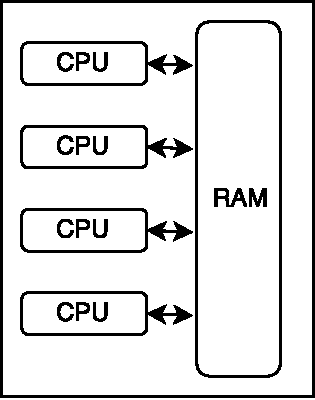
\includegraphics[scale=0.6]{parallel.pdf}
		\subcaption{\label{subfigure_a}}
	\end{subfigure}
	\begin{subfigure}{0.5\textwidth}
		\centering
		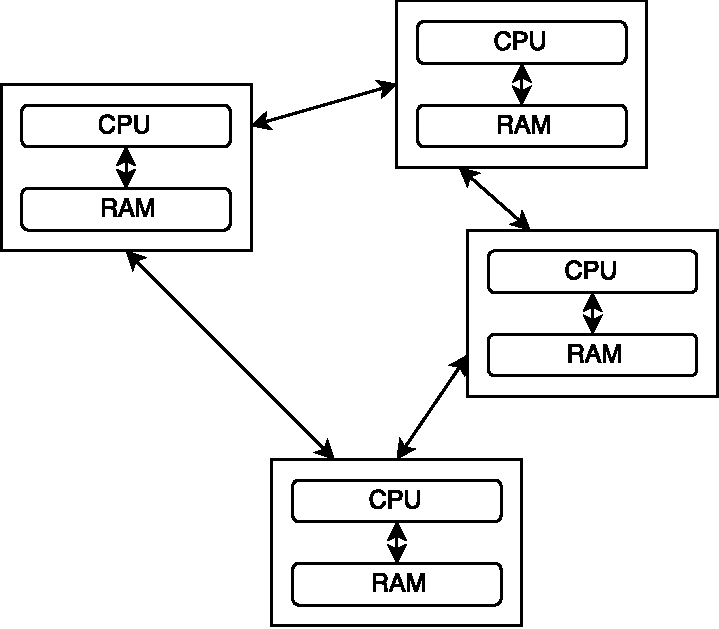
\includegraphics[scale=0.5]{distributed.pdf}
		\subcaption{\label{subfigure_b}}
	\end{subfigure}
	\begin{subfigure}{0.6\textwidth}
		\centering
		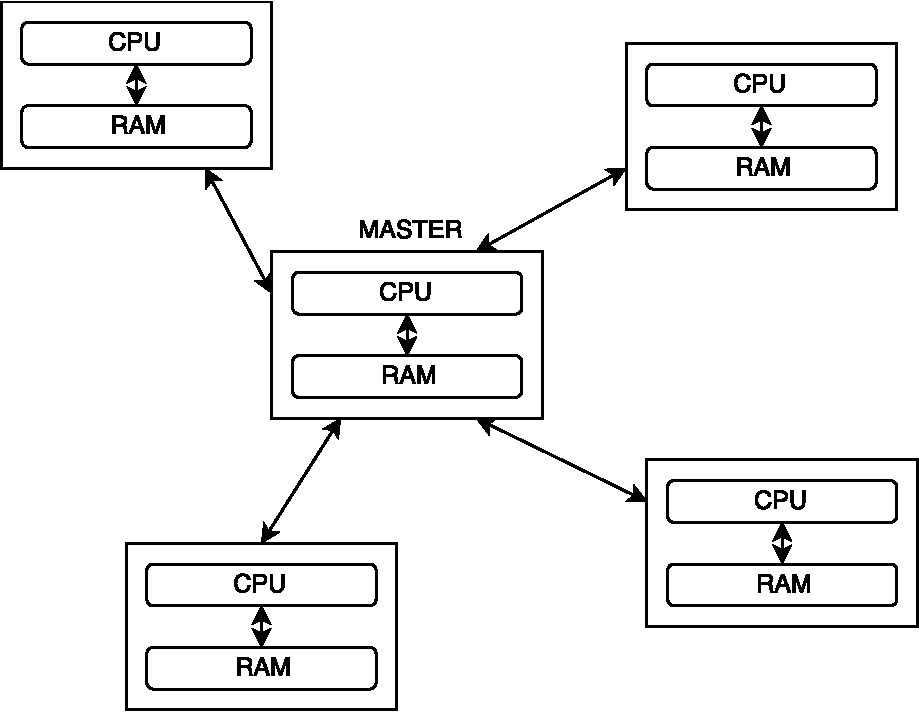
\includegraphics[scale=0.5]{decentralized.pdf}
		\subcaption{\label{subfigure_c}}
	\end{subfigure}
	
	\caption{\label{fig:concurrentVsParalell}Wizualizacja różnicy pomiędzy systemem równoległym \protect\subref{subfigure_a}, rozproszonym \protect\subref{subfigure_b} i zdecentralizowanym \protect\subref{subfigure_c}.}

\end{figure}

\section{Narzędzia rozpraszania danych}
\label{sec:narzedzia}
Najbardziej istotnym problemem z dziedziny rozproszenia dla systemu dHTTP jest rozproszenie danych -- próba propagowania informacji pomiędzy wiele węzłów sieci, w celach takich jak podniesienie wydajności, obniżenie kosztów, zwiększenie dostępności czy zapewnienie trwałości informacji.

Dobrym przykładem rozwiązania rozproszonego w operacjach na danych jest system kontroli wersji \texttt{git}.
Został stworzony przez Linusa Torvaldsa, autora jądra Linux, jako otwarta alternatywa dla systemu BitKeeper, który wycofał z dystrybucji darmową wersję swojej aplikacji projektom open source.
\texttt{git} jest projektem czysto rozproszonym -- każdy użytkownik posiada kompletną kopię repozytorium, z informacjami o wszystkich zmianach i ich autorach, na której może wykonywać operacje w trybie offline; nie jest uzależniony od istnienia centralnego serwera (choć jego stosowanie jest powszechne; każdy użytkownik o aktualnej wersji repozytorium mógłby jednak pełnić jego rolę), a zmiany mogą być propagowane na różne sposoby, takie jak email czy przekazywanie łat w formie tekstowej. Dzięki swojej wydajności i silne zdecentralizowanemu designowi, \texttt{git} jest chętnie wybieranym rozwiązaniem nie tylko w środowiskach programistów, a w środowiskach profesjonalnych wypiera konkurencyjne rozwiązania, takie jak Apache Subversion czy CVS \cite{ram2013git}.

Nie zawsze jednak motywacje stojące za rozpraszaniem danych poza centralne serwery były szczytne. Duży wpływ na rozwój technik stosowanych obecnie -- w tym wykorzystywanych przez dHTTP -- mają rozwiązania rozpowszechnione głównie przez piractwo komputerowe. Systemy peer-to-peer -- polegające na współpracy równorzędnych węzłów -- zostały spopularyzowane dzięki aplikacji Napster, która w roku 2001 zgromadziła około 80 milionów użytkowników. Zaprojektowana jako system współdzielenia plików, wyspecjalizowała się w łatwym udostępnianiu plików MP3. Napster wzburzył wiele kontrowersji -- w systemie pojawiały się niewydane jeszcze utwory znanych artystów, prowadząc do milionowych strat i procesu, który pogrążył działanie systemu.
Problemem Napstera była architektura oparta o centralny serwer indeksujący -- każdy podpięty węzeł informował o posiadanych przez siebie plikach, a punkt centralny był niezbędny do przeszukiwania bazy plików i przekazywania poleceń pobrania innym węzłom. To rozwiązanie stanowiło słaby punkt sieci, i pozwoliło obciążyć twórców programu odpowiedzialnością za szerzone w nim treści.

Błędy Napstera zostały zauważone przy kolejnych projektach tego typu. Gnutella, chcąc uniknąć istnienia {\em single point of failure}\footnote{Punkt sieci, którego awaria powoduje zatrzymanie pracy całego systemu.}, działała na zasadzie rozgłaszania poleceń użytkowników do wszystkich maszyn w sieci, co owocowało jednak drastycznym spadkiem wydajności \cite{measuringNapsterGnutella}.

Alternatywne podejście podjęte zostało przez sieć Freenet, gdzie zastosowano heurystyczny routing oparty o klucze; każdy plik otrzymuje klucz, a podobne klucze lokowane były na zbliżonych do siebie węzłach, dzięki czemu przeszukiwanie sieci nie wymagało punktu centralnego, a polecenia kierowane były w sposób niewymagający wielu przeskoków. Niestety, ta metoda nie gwarantowała znalezienia danych \cite{searchingInSmallWorld}.

Chcąc pogodzić kwestie bezpieczeństwa, wydajności i spójności systemu, rozpoczęte zostały intensywne prace nad rozproszonymi tablicami haszującymi (distributed hash table -- \textbf{DHT}). To rozwiązanie pozwala na trzymanie dużych ilości informacji w sposób kompletnie rozproszony -- wszystkie węzły sieci znają zestaw kluczy, stanowiących {\em de facto} adresy danych, pozwalające użytkownikom na przeszukania; znalezienie węzłów trzymających właściwe dane jest umożliwione dzięki ich opartemu o klucze sposobie identyfikacji. Choć przechowywanie tablicy DHT jest dodatkowym kosztem obciążającym system, i wymagane jest ustalenie wspólnych funkcji hashujących, przy właściwej konfiguracji to rozwiązanie pozwala na obsługę całej sieci danych bez serwerów pośredniczących.

\section{Podstawa projektu}
\label{sec:podstawaProjektu}

Wspomniane rozwiązania stanowią kanwę dla projektu IPFS \cite{ipfsWP}, który stara się tworzyć efektywny, realnie rozproszony system plików, obsługujący gigantyczne zasoby danych z niskimi latencjami, redundancją danych i bez wymogu zaufania uczestnikom sieci.  Dane przechowywane są w drzewie Merkla, dzięki czemu przeszukiwanie sieci ma niską złożoność obliczeniową. Projekt skupia się na warstwie infrastruktury – po stronie użytkowej przypomina nieco system kontroli wersji \texttt{git}, a dane indeksowane są dzięki sumom kontrolnym, i ich adresy to wieloznakowe hashe. Takie podejście doskonale sprawdza się w skryptach i przy pracach prowadzonych przez ludzi obytych z tego typu narzędziami, nie jest to jednak system przyjazny użytkownikom domowym.

Celem tej pracy jest adaptacja dokonań projektu IPFS jako {\em przezroczysty} system wsparcia HTTP. W swoim założeniu, system nie może próbować zastąpić istniejących rozwiązań. Internet w obecnym kształcie nie jest gotowy na rewolucje – przykładem może być poziom przyjęcia się IPv6 \cite{googleipv6}, następnej generacji protokołu IP, która ma między innymi rozwiązać problem rozmiaru puli adresów. Brak realnej kompatybilności wstecznej sprawia, że konieczne są rozwiązania przejściowe. dHTTP jest bardziej nakładką, rozwinięciem obecnych rozwiązań -- współżyje z nimi -- co daje perspektywy spokojnego przyjęcia takiego rozwiązania przez rynek.

IPFS posiada wzorcową implementację w języku Go, i jest podstawą stosu sieciowego \texttt{libp2p}. Zbiór bibliotek udostępniony w projekcie \texttt{js-libp2p} stanowi fundament projektu dHTTP, który, dzięki natywnej implementacji w JavaScripcie, może być w pełni uruchamialny z poziomu przeglądarki.

\chapter{Projektowanie i implementacja}
\label{cha:implementacja}

Nakreślony problem -- rozproszonego systemu, który dzięki propagacji danych między użytkownikami obniży obciążenie serwerów sieci Web -- stawia wiele wyzwań projektowych i architektonicznych.

\section{Wymagania funkcjonalne}
\label{sec:funkcjonalnosc}

System dHTTP, z punktu widzenia użytkownika, ma spełniać jedną funkcjonalność: utrzymać lub poprawić płynność dostępu do interesujących go witryn internetowych, nie wpływając na ich treść i nie naruszając prywatności.

Projekt udostępnia interfejs zapewniający dostęp do statystyk, a także preferencji użytkownika. Udostępnione preferencje dotyczą: stopnia działania aplikacji w tle, trybów propagacji i przechowywania danych.

\begin{figure}[h]
	\centering
    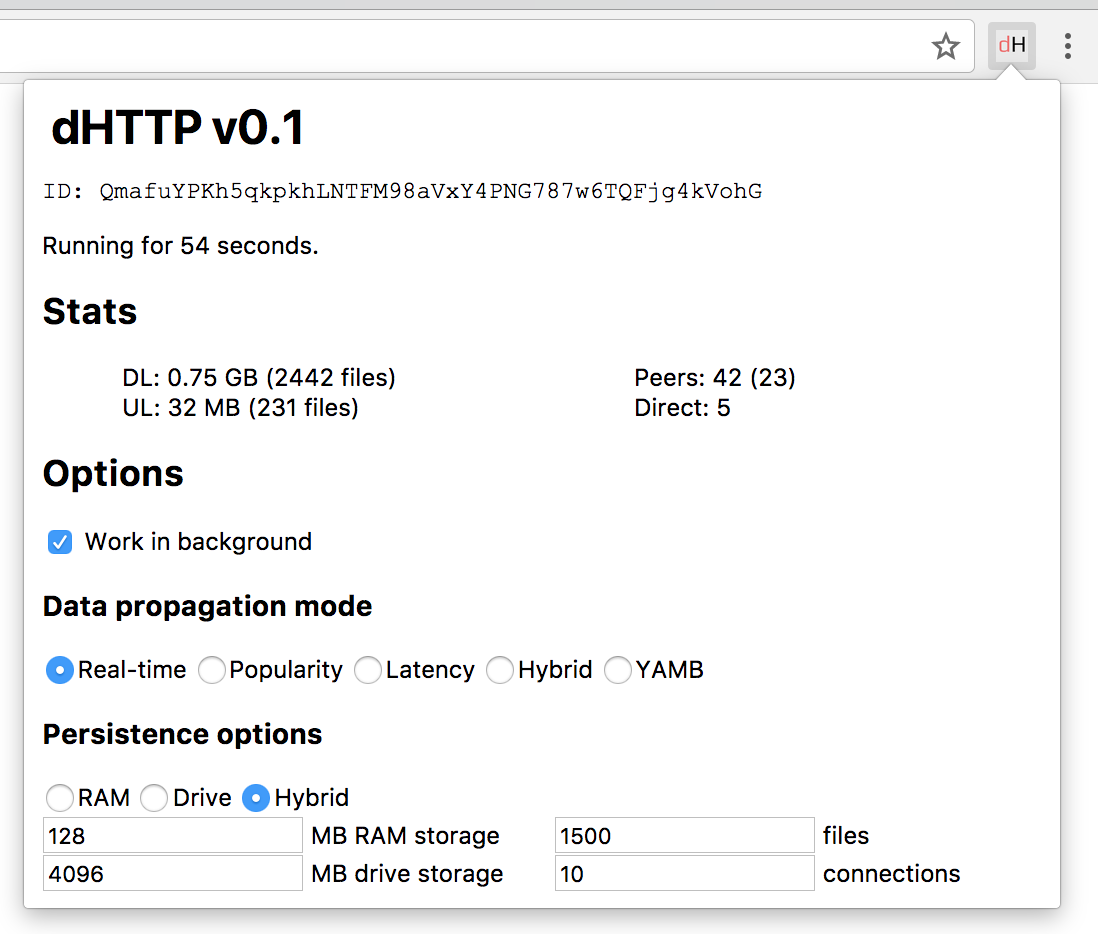
\includegraphics[scale=0.5]{dhttp-initial-interface.png}
	
	\caption{\label{fig:initialInterface} Wstępna implementacja interfejsu operacji dla systemu dHTTP: pop-up dostarczany przez wtyczkę do przeglądarki Google Chrome pozwala na obserwację statystyk i zmianę preferencji.}
\end{figure}

Wymogiem dla projektu, koniecznym z racji potrzeby prostej automatyzacji rozrostu sieci, jest tryb niezależny aplikacji -- {\em headless mode} -- pozwalający na wystartowanie niezależnego węzła jednym poleceniem. Istotnym jest, aby węzeł tego typu udostępniał statystyki użycia i wstępną konfigurację przy użyciu poleceń interfejsu konsolowego, pozwalając jednak na funkcjonalne uruchomienie z domyślną konfiguracją.


\section{Definicje, architektura i technologie}
\label{sec:zalozeniaProjektu}

\subsection{Słownik pojęć}

W celu uniknięcia niejednoznaczności w dalszym toku pracy, zdefiniowane zostaną następujące pojęcia:

\begin{itemize}
    \item \textbf{węzeł} -- pojedynczy, autonomiczny element systemu, który wykorzystuje komunikację sieciową w celu rozgłaszania i pobierania danych;
    \item \textbf{klient} -- węzeł, który pobiera dane w celach użytkowych, zaimplementowany w wersji dedykowanej użytkownikowi końcowemu;
    \item \textbf{klaster} -- zbiór węzłów, który posiada informacje i ścieżki komunikacyjne pozwalające efektywnie na wymianę informacji pomiędzy każdym z nich;
    \item \textbf{metadane klastra} -- ustrukturyzowane informacje wymieniane pomiędzy węzłami w celu ustalenia stanu i optymalizacji działania klastra;
    \item \textbf{metadane pliku} -- ustrukturyzowane informacje wymieniane między węzłami w celu propagacji i umożliwienia wymiany faktycznych danych plikowych;
\end{itemize}


\subsection{Koncept architektury}

Z punktu widzenia klastra, koncepty węzła i klienta są jednoznaczne i równorzędne -- wszystkie wyposażone są we wspólne mechanizmy komunikacji, i protokół wymiany danych między nimi działa na niezmienionej zasadzie. Wspólnie budować będą rozproszoną tablicę haszującą (DHT), która pozwoli na dostęp do metadanych klastra informujących o cechach poszczególnych węzłów oraz metadanych plików, przyspieszając proces ich identyfikacji i zapewniając bezpieczeństwo oraz spójność danych.

\subsection{Wykorzystane technologie i narzędzia}
\label{sec:techNTools}

Budowa kompletnego stosu technologicznego dla projektu o takich wymaganiach przez lata pozostawała problemem nietrywialnym. Paradygmaty programowania specjalizowane w podejściu obiektowym wspierały budowę monolitów, a komunikacja klient-serwer często polegała na tworzeniu dużej ilości poleceń, bez skupienia na wydajności takich rozwiązań.

Dużą zmianą w tej kwestii jest rozwój \texttt{libp2p}, stanowiący efekt długotrwałej pracy nad zrozumieniem stosu sieciowego Internetu, zbiór protokołów i wyprowadzonych zeń narzędzi, mechanik i interfejsów, pozwalających na ich podstawie budować własne, kompleksowe rozwiązania \cite{libp2p-specs}.

\texttt{libp2p} stanowi względnie wysokopoziomową podstawę projektu dHTTP. To właśnie na efektach pracy tego projektu opiera się warstwa tworzenia i komunikacji węzłów, budująca klaster dHTTP. Implementacja \texttt{js-libp2p} udostępnia moduły niezbędne w komunikacji sieciowej, łączeniu strumieni różnych protokołów, wykrywaniu nowych węzłów, propagowaniu informacji o stanie sieci czy wreszcie budowaniu rozproszonej tablicy haszującej, stanowiącej bazę metadanych klastra i plików.

Nie bez wpływu pozostaje rozwój przeglądarek internetowych; współcześnie udostępniają one kompleksowe API, pozwalające rozwijać wtyczki zmieniające zawartość stron internetowych, z uwzględnieniem kwestii wydajności i bezpieczeństwa. Istotne jest również wsparcie dla nowych technik komunikacji takich jak {\em WebSockets}, pozwalającej na wymianę informacji w czasie rzeczywistym, dzięki utrzymywaniu dwustronnie interaktywnej sesji TCP pomiędzy przeglądarką i serwerem. W ramach tej pracy rozwinięta została wtyczka dla przeglądarki Google Chrome. Wybór ten podyktowany został znaczną przewagą Chrome -- w chwili pisania tej pracy, udział Chrome w rynku przeglądarek na komputerach osobistych wynosił ponad 64\% \cite{chromeStats}. Prace i testy przeprowadzono przy użyciu 64-bitowego Google Chrome w wersji 63.0, na platformie macOS w wersji 10.13.2.

Za powstanie {\em headless} dHTTP w znacznej części odpowiada Node.js -- środowisko uruchomieniowe pozwalające na uruchamianie kodu JavaScript po stronie serwerowej.  Narzędzia, takie jak \texttt{npm} i Browserify, pozwalają z kolei na wykorzystywanie serwerowego kodu JavaScriptu w kodzie klienckim. Dzięki możliwości rozwoju obu aplikacji przy użyciu tego samego języka programowania i powyższym rozwiązaniom, znaczna część  kodu aplikacji może być współdzielona. {\em Headless} dHTTP testowane było przy użyciu \texttt{node} w wersji v8.9.1, na platformie macOS oraz Amazon Linux AMI.

\subsection{Paradygmaty i koncepcje}
Istotą projektu dHTTP jest reagowanie na zapytania i komunikacja pomiędzy węzłami. Ponadto, projekt działać będzie w środowisku JavaScriptowym -- język ten (poza {\em web workers} -- rozwiązaniem polegającymi na delegacji obliczeń do wydzielonego środowiska, patrz: \cite{webWorkers}) uruchamiany jest jednowątkowo. W podejściu proceduralnym może to powodować problemy związane z blokowaniem się wydarzeń; jest to dotkliwe zwłaszcza w przypadku interfejsów użytkownika, które w takiej sytuacji tracą responsywność. Poniższe sekcje zawierają omówienie związanym z tych praktyk, stosowanych w projekcie dHTTP.


\subsubsection{Asynchroniczność}
Podstawowym rozwiązaniem stosowanym w języku JavaScript, pozwalającym na wykonanie w środowisku jednowątkowym, jest model współbieżności oparty o tzw {\em event loop}. Wywołania funkcji odkładane są na stosie, podczas gdy kolejne wiadomości są wkładane do kolejki FIFO. Podstawowym założeniem jest nigdy nie blokować -- jeśli jakieś wywołanie wymaga konkretnej reakcji, definiowanej przez użytkownika, należy nasłuchiwać wydarzeń lub użyć wywołań zwrotnych (\texttt{callback}).

\begin{lstlisting}[language=javascript]
    function foo(callback) {
        var a = someWaitingOperation()
        callback(a)
    }

    foo((a) => print(a))
    console.log('Hello, world!')
\end{lstlisting}

W powyższym przykładzie warto zauważyć, że wywołanie \texttt{console.log(...)} będzie miało miejsce natychmiast po zawołaniu funkcji foo -- jest więc bardzo prawdopodobnym, że efekt jego pracy widoczny będzie przed zawołaniem funkcji \texttt{callback}.

Asynchroniczne odwołania są kluczowe w przypadku wydarzeń takich jak oczekiwanie na odpowiedź serwera; czekając, program może wykonywać następne polecenia, a reakcja na odpowiedź zostanie wpleciona w tok pracy aplikacji.

\subsubsection{Event-driven architecture}
Pozioma oś modelu współbieżności JavaScriptu zapewnia natywne wsparcie dla reakcji na wydarzenia. W celu nasłuchiwania wydarzenia, należy zarejestrować jego obserwatora ({\em listener}) stosując z reguły składnię zbliżoną do:
\begin{lstlisting}[language=javascript]
    a.addEventListener('click', ()=> {
        console.log('Button clicked!')
    })
\end{lstlisting}

W powyższym przykładzie zaprezentowano rejestrację reakcji na kliknięcie w przycisk. Jeżeli dana sytuacja nastąpi, wiadomość wysłana zostanie na kolejkę, co w momencie jej napotkania doprowadzi do wrzucenia na stos zarejestrowanej funkcji.

\begin{figure}[h]

    \centering
    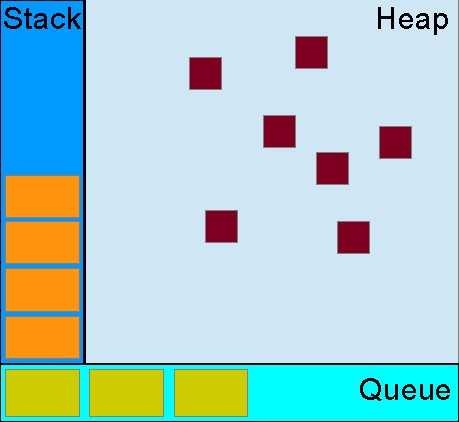
\includegraphics[scale=0.6]{js-concurrency.pdf}

	\caption{Wizualizacja modelu współbieżności języka JavaScript -- widać stos funkcji (oś pionowa) i kolejkę wydarzeń (oś pozioma). Pomiędzy nimi znajduje się współdzielona sterta, zapewniająca dostęp do danych. Źródło: \cite{eventLoop}}

\end{figure}

\subsubsection{Strumienie}

Node.js przeniósł środowisko JavaScript, którego dotychczasowym targetem były lekkie rozwiązania klienckie, na poziom serwerowy, w którym niektóre operacje są długotrwałe, mają przerwy w wywołaniach i nierzadko wymagają informowania o postępach (przykładem może być utrzymanie połączenia sieciowego, czy odczyt standardowego wyjścia). Choć jest możliwym implementacja tego typu rozwiązań  wywołaniami zwrotnymi, czytelność i utrzymywalność takiego kodu drastycznie spada -- przepływ logiki programu staje się trudny do wyśledzenia.

Z pomocą przychodzą strumienie \cite{nodeStreamAPI}. Strumienie nakładają abstrakcję, która pozwala intuicyjnie czytać (dla strumieni \texttt{Readable}) wrzucać (w przypadku \texttt{Writable}), a także transformować (\texttt{Transform}) przekazywane wartości.

\begin{lstlisting}[language=javascript]
// Przykład nawiązywania połączenia w metaprotokole dHTTP
dhttpClient.node.dial(peerInfo, '/dhttp/meta/0.1', (err, connStream) => {
    // connStream to przykład strumienia Duplex - pozwala zarówno na zapis, jak i odczyt.
    // zapis do connStream
    connStream.write("Let's talk")
    // jeśli w strumieniu pojawią się dane, nastąpi wywołanie funkcji callback. Warto zauważyć, że to wywołanie może nastąpić zarówno przed, jak i po zawołaniu write -- zależy od stanu strumienia, który może otrzymywać dane w innych miejscach programu
    connStream.on('data', (data) => {
        callback(JSON.parse(data))
    })
}


// Przykład uruchamiania serwera HTTP w node.js dzięki "require('http')"
http.createServer((req, res) => {
    // Przekazanie strumienia req strumieniowi request, który następnie zostanie przekazany do res. W efekcie zadziałamy jako najprostsze proxy - otrzymamy dane o oryginalnym zapytaniu, wywołamy je z punktu widzenia serwera, i przekażemy wynik w ramach odpowiedzi.
    req.pipe(request(req.url)).pipe(res)
}).listen(34887)
\end{lstlisting}

Powyższy przykład, stanowiący część kodu dHTTP, pokazuje istotny koncept {\em potoków} (ang. {\em pipe}). Potoki pozwalają łączyć strumienie w sposób analogiczny do strumieni znanych z systemów Uniksowych: odczytane wartości można przekazać kolejnemu strumieniowi, który może zamienić je na inne wartości, aż w końcu wynik pracy zostanie zapisany w strumieniu odpowiedzi. Tego typu operacje stanowią podstawę przemian stosowanych w dHTTP.

Podkreślić należy również pozytywny wpływ strumieni na wydajność -- ta abstrakcja pozwala operować na plikach przy użyciu buforów w sposób niewidoczny: przykładowo, aby wysłać duży obrazek nie przechowując go w całości w pamięci, wystarczy utworzyć strumień pliku i przepotokować go do strumienia wyjściowego.

\begin{lstlisting}[language=javascript]
    var fileStream =  fs.createReadStream(filePath);
    fileStream.pipe(connStream)
    //kiedy strumień pliku się zakończy, nastąpi zamknięcie połączenia aby poinformować odbiorcę, że nic już na niego nie czeka
    fileStream.on('finish', ()=> connStream.close())
\end{lstlisting}

\section{Interfejs \texttt{dhttp.js}}

Podstawę logiki systemu stanowi plik \texttt{dhttp.js}. Jest on interfejsem łączącym szkielet aplikacji i stronę użytkową, pozwalającym na dostęp do informacji na temat sposobu działania węzła, a także wykonywanie operacji w sieci dHTTP.

\texttt{dhttp.js} operuje na dwóch protokołach:

\begin{itemize}
    \item \texttt{/dhttp/meta/0.1} -- {\em metaprotokół}, stanowi podstawę szkieletu systemu dHTTP. Informuje o dostępnych węzłach i plikach, obciążeniu sieci, a także następujących na bieżąco zmianach. Konwencją podjętą dla {\em metaprotokołu} jest powszechna propagacja danych -- przykładowo, jeśli następuje połączenie z nowym węzłem,  należy wysłać mu listę posiadanych plików, a jeśli planowane jest opuszczenie sieci, trzeba poinformować o tym fakcie podłączonych sąsiadów. Dzięki temu podejściu każdy węzeł posiada zbiór informacji na temat otoczenia, pozwalający na szybsze podejmowanie decyzji.

    \item \texttt{/dhttp/data/0.1} -- {\em protokół danych}, stanowi system przesyłu docelowych plików w dHTTP. Zorientowany strumieniowo, przesyła zgromadzone pliki w ich oryginalnym formacie. Może zostać rozszerzony o obsługę zapytań cząstkowych -- tak, aby duże pliki pobierać częściami od swoich sąsiadów.
\end{itemize}
Ponadto, \texttt{dhttp.js} wykorzystuje wbudowane {\em mechanizmy odkryć} \texttt{libp2p} w celu wykrywania sąsiadów i zmian sieci.



\subsection{Warstwa sieciowa}
Warto zaznaczyć, że rozwiązania opisywane w powyższej sekcji jako {\em protokół} są wysokopoziomową nakładką na warstwę sieciową. Jak zatem węzły nawiązują połączenie?

Połączenia w sieci peer-to-peer są znacznie utrudnione przez \textbf{ Network Address Translation} (NAT). NAT jest techniką stosowaną przez routery, polegającą na zmianie adresów i portów IP w toku przesyłu danych w celu udostępnienia węzłom sieci prywatnych dostępu do internetu przy użyciu jednego adresu. Gdy użytkownik za „maskaradą” (jak bywa określany NAT) wykonuje zapytania, serwery widzą adres IP pierwszego routera, który posiada publiczny adres sieciowy. Odpowiedzi są możliwe dzięki informacjom przechowywanym przez routery prowadzące ten typ komunikacji.

Jest to konieczność w obliczu wyczerpanej puli adresów IPv4, prowadzi jednak do sytuacji, w której otwarcie bezpośredniego łącza pomiędzy dwoma użytkownikami końcowymi jest z reguły niemożliwe -- nie ma możliwości odpytania adresu IP końcowego komputera.

W celu poradzenia sobie z tym problemem, dHTTP wykorzystuje bibliotekę \texttt{js-libp2p-webrtc-star}. To rozwiązanie działa na zasadzie serwera spotkań ({\em Rendezvous Server}), który stanowi swoisty przekaźnik i pozwala na rejestrację węzłów. Dzięki temu, jest jednocześnie odpowiedzialny za warstwę transportu jak i {\em mechanizm odkryć}.

\begin{figure}[h]
        \centering
        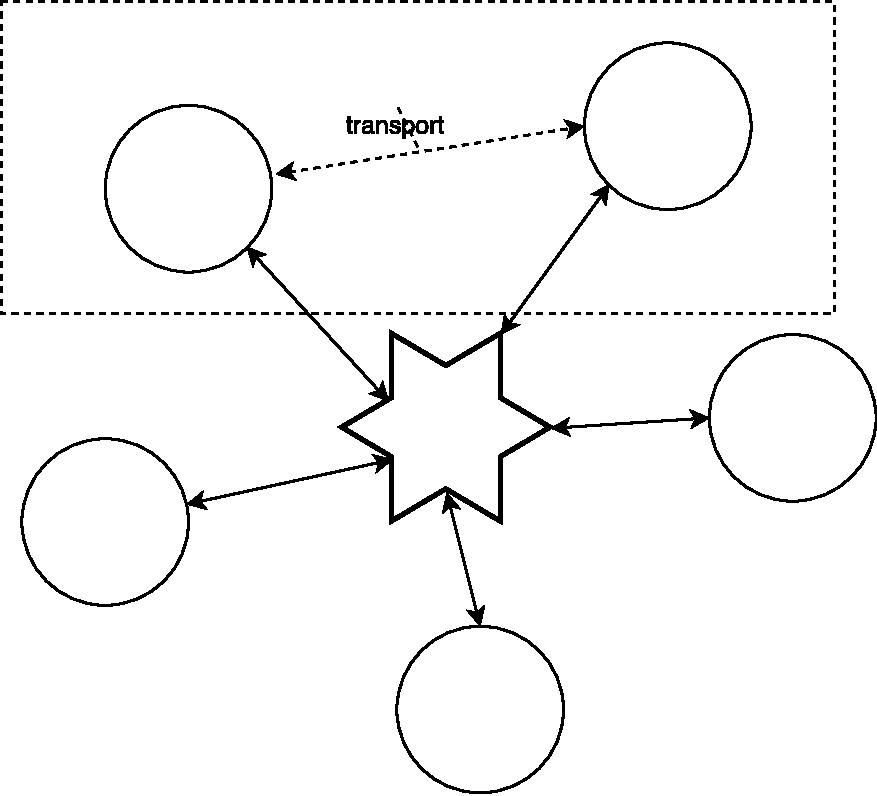
\includegraphics[scale=0.5]{webrtc-star.pdf}
    
        \caption{Wizualizacja sieci opartej o \texttt{js-libp2p-webrtc-star}, z przykładem wirtualnego połączenia transportowego pomiędzy dwoma węzłami.}
        \label{fig:webrtc-star}
\end{figure}

Niestety, stawia to pod znakiem zapytania rozproszenie systemu -- jak widać na rys. \ref{fig:webrtc-star}, obecnie system przypomina bardziej scentralizowaną topologię gwiazdy niż system faktycznie rozproszony. Obciąża też {\em Rendezvous Server} koniecznością przekazywania treści. Jest to jednak rozwiązanie przejściowe i na chwilę obecną konieczne -- \texttt{js-libp2p} w czasie tworzenia tego projektu nie udostępnia innych metod trawersowania NAT-u.

Warto dodać, że w przypadku sieci opartej wyłącznie o węzły w sieci lokalnej możliwe jest stosowanie tzw. Multicast DNS, który nie potrzebuje żadnego punktu centralnego; w przypadku serwerów posiadających publiczne adresy IP, możliwe staje się użycie list adresów utrzymywanych przez serwery śledzące -- trackery -- oba rozwiązania pozwalają na bezpośredni transport pomiędzy węzłami i nie wymagają zmiany logiki systemu (\cite{discoverylibp2p}).

\subsection{Struktura metadanych}
\label{sub:metadata}

Metadane przesyłane przy użyciu \texttt{/dhttp/meta/0.1} to podstawa przepływu danych w systemie. Wykorzystywane do budowania wspólnej bazy wiedzy na temat sieci, składać się muszą z lekkich struktur i jasnych komunikatów.

Podstawowe zapytanie \texttt{/dhttp/meta/0.1} wygląda następująco:

\begin{lstlisting}[language=javascript]
    {
        type: "echo",
        peerId: dhttpClient.node.peerInfo.id.toB58String(),
        text: "Hello, node."
    }
\end{lstlisting}

Omówienie zapytań i odpowiedzi jest zawarte w rozdziale \ref{sec:api}.


\section{API}
\label{sec:api}

W tej sekcji szczegółowo opisane zostały udostępnione przez \texttt{dhttp.js} funkcje i mechanizmy związane ze strukturami i przepływami danych pomiędzy węzłami. Ogólny przepływ informacji systemu zawiera się w podsekcji \ref{sec:transportAlgorithm}, opisującej cykl życia węzła.

Podstawowym założeniem jest istnienie singletona\footnote{Możliwość tworzenia obiektu ograniczona jest do pojedynczej, globalnie dostępnej instancji.} \texttt{dhttpClient}, który przy rozruchu aplikacji inicjalizuje węzeł sieci. Wszelkie odwołania do działania węzła powinny polegać na rejestrowaniu wydarzeń i wywoływaniu funkcji globalnego obiektu \texttt{dhttpClient}.

\subsection{Struktury danych}
W celu poprawy wydajności i uproszczenia przepływów w aplikacji, dHTTP oferuje kilka struktur informujących o dostępności danych.

Typy struktur jak i funkcje oferowane przez \texttt{js-libp2p}, do których odnosi się poniższe API, opisane są na stronie projektu: \cite{libp2pReadme}.

\subsubsection{Struktury podstawowe}
\begin{itemize}
    \item \textbf{\texttt{PeerId}} -- \texttt{String} zawierający ID węzła sieci, uzyskane dzięki zawołaniu \texttt{PeerInfo.id.toB58String()}
    \item \textbf{\texttt{RequestURL}} -- \texttt{String} zawierający ścieżkę zapytania klienckiego. Jeśli klient odpyta nasz serwer na adresie \texttt{http://localhost:34887/http://example.com/script.js}, instancja \texttt{RequestURL} zawierać będzie \texttt{http://example.com/script.js}.
    \item \textbf{\texttt{popularityIndex}} -- \texttt{Integer} określający popularność danego pliku z perspektywy posiadającego go węzła.
    \item \textbf{\texttt{Data}} -- serializowalny obiekt zawierający dane przesyłane w ramach metaprotokołu, zgodne z formatami zdefiniowanymi w \ref{sub:metaprotocolMessages}.
\end{itemize}

% 

\subsubsection{\texttt{filesInNetwork}}
\begin{lstlisting}[language=javascript]
filesInNetwork: {
        "http://example.com/file.jpg": { // RequestURL
            nodes: {
                PeerId: {
                    popularityIndex: Int,
                }
            }
            popularityIndex: Int
        },
        "http://example.com/script.js" : {...}
    }
\end{lstlisting}
\texttt{filesInNetwork} jest strukturą odpytywaną przy połączeniu klienckim. Stanowi pierwszy punkt wejścia do sieci, i zoptymalizowany jest pod szybkie przeszukanie i weryfikację, czy plik jest dostępny przy użyciu dHTTP.

Poszczególne elementy indeksowane są poprzez adresy URL zasobów pobieranych przez klienta (\texttt{ReqestURL}).

\textbf{Pola:}
\begin{itemize}
    \item \textbf{\texttt{nodes}} -- mapa zawierająca informacje tych klientów, którzy posiadają dostęp do danego pliku.
    \item \textbf{\texttt{popularityIndex}} -- liczba całkowita określająca popularność pliku z perspektywy tego węzła. Może być wymieniana z innymi węzłami sieci w celu optymalizacji obciążenia -- ułatwi węzłowi odpytywanemu decyzję na temat przekazania połączenia do najmniej zajętego sąsiada.
\end{itemize}

% 

\subsubsection{\texttt{swarm}}
\begin{lstlisting}[language=javascript]
swarm: { 
    nodes: { 
        QmVxxoRFLR8VjbqeVer9Z9DqCJoJT36c9Uomd9AtP8NBx6: // PeerId
            PeerInfo {...}
    } 
}
\end{lstlisting}
\texttt{swarm} jest strukturą utrzymującą informacje na temat wszystkich węzłów, które są bezpośrednio podłączone do obecnego. Reprezentuje więc swoisty {\em lokalny klaster}, z całością którego można nawiązywać połączenia.

\textbf{Pola:}
\begin{itemize}
    \item \textbf{\texttt{nodes}} -- obiekt, w którym poszczególne elementy reprezentują \texttt{PeerInfo} -- kompleksowy zbiór informacji z API \texttt{js-libp2p}, pozwalający na nawiązywanie połączeń.
\end{itemize}

% 

\subsubsection{\texttt{stats}}
\begin{lstlisting}[language=javascript]
stats: {
    downloaded: {bytes: 0, files: 0},
    fetched: {bytes: 0, files: 0},
    uploaded: {bytes: 0, files: 0},
}
\end{lstlisting}
\texttt{stats} gromadzi statystyki zużycia sieci przez obecny węzeł.

\textbf{Pola:}
\begin{itemize}
    \item \textbf{\texttt{downloaded}} -- ile danych pobrano z perspektywy klienta.
    \item \textbf{\texttt{fetched}} -- ile danych pobrano w tle -- podczas operacji niezwiązanych bezpośrednio z działania użytkownika, lecz podjętych w celach optymalizacyjnych.
    \item \textbf{\texttt{uploaded}} -- ile danych wysłano do innych węzłów podczas działań optymalizacyjnych i propagacji danych w systemie.
\end{itemize}

% 

\subsubsection{\texttt{node}}
\begin{lstlisting}[language=javascript]
    node: Node {protocols: {...}, peerInfo: PeerInfo, ...}
\end{lstlisting}
\texttt{node} jest obiektem pozwalającym na bezpośredni dostęp do reprezentacji danego węzła w warstwie \texttt{js-libp2p}. Pozwala na wykonywanie połączeń i propagację danych z poziomu innych funkcji dHTTP. Szczegóły zawarte w dokumentacji projektu \cite{libp2pReadme}.

% 

\subsubsection{\texttt{storage}}
\begin{lstlisting}[language=javascript]
storage: {
    quotas: {
        RAM: {
            files: 0, megabytes: 0
        },
        drive: {
            files: 0, megabytes: 0
        }
    },
    RAMFiles: {
        files: {
            "http://example.com/logo.png": { // RequestURL
                value: Blob
            },
            "http://example.com/logoLocalStorage.png": { ... },
            ...
        }
    },
    driveFiles: {
        files: {
            "http://example.com/onDrive.png": { // RequestURL
                path: "/files/http:++example.com+onDrive.png"
            },
            "http://example.com/onDrive2.png": { ... },
            ...
        }
    }
}
\end{lstlisting}
\texttt{storage} nakłada warstwę abstrakcji na obsługę plików utrzymywanych przez węzeł, która automatyzuje proces wyboru rodzaju pamięci dla zapisu oraz odczytu danych.

\textbf{Pola:}
\begin{itemize}
    \item \textbf{\texttt{quotas}} -- obiekt który zawiera w sobie konfigurację ograniczeń pamięci. Dla wartości \texttt{0} nie istnieją żadne ograniczenia; wartość \texttt{-1} oznacza zakaz korzystania z danego rodzaju pamięci.
    \item \textbf{\texttt{RAMFiles}} -- zbiór wszystkich plików przechowywanych w pamięci RAM.
    \subitem  \textbf{\texttt{value}} -- plik trzymany w formacie binarnym, gotowy do strumieniowego przesłania użytkownikowi końcowemu.
    \item \textbf{\texttt{driveFiles}} -- zbiór wszystkich plików przechowywanych w systemie plików użytkownika.
    \subitem  \textbf{\texttt{value}} -- względna ścieżka do pliku, który zawiera dany zasób.
\end{itemize}


%  FUNKCJE

\subsection{Funkcje}
\label{sub:functions}

Dzięki szeregowi udostępnionych funkcji, dHTTP umożliwia wysokopoziomowe, asynchroniczne podejście do informacji o systemie i zawartości plików. Poniżej zostały zawarte opisy najważniejszych z nich.

\subsubsection{\texttt{filesAvailable/0}}
\begin{lstlisting}[language=javascript]
    filesAvailable: function() -> ({RequestURL: {PopularityIndex}})
\end{lstlisting}
\texttt{filesAvailable} jest funkcją stanowiącą wykaz wszystkich plików udostępnionych przez dany węzeł. Nie stosuje rozróżnienia na dane dostępne w RAMie czy na dysku -- ta optymalizacja pozostaje na poziomie poszczególnych węzłów, aby nie obciążać wszystkich klientów sieci.

\textbf{Wartość zwracana:}
Mapa \texttt{RequestURL} obsługiwanych przez dany węzeł na ich \texttt{PopularityIndex}.

% \textbf{Przykład wywołania:}
% \begin{lstlisting}[language=javascript]
%     introductoryData: function () {
%     return {
%         type: "introduction",
%         peerId: dhttpClient.node.peerInfo.id.toB58String(),
%         files: dhttpClient.filesAvailable()
%     }
% }
% \end{lstlisting}


% 

\subsubsection{\texttt{dialNode/3}}
\begin{lstlisting}[language=javascript]
    dialNode: function(PeerInfo, Data, (ResponseData) -> ()) -> ()
\end{lstlisting}
\texttt{dialNode} pozwala na wykonanie połączenia do istniejącego węzła w celu przesłania mu metadanych projektu. W ramach danych, wysłane mogą zostać serializowane obiekty komunikatów, opisane szczegółowo w sekcji \ref{sub:metaprotocolMessages}.

\textbf{Parametry:}
\begin{itemize}
    \item \textbf{\texttt{PeerInfo}} -- obiekt \texttt{PeerInfo} węzła do którego ma zostać wysłana wiadomość
    \item \textbf{\texttt{Data}} -- serializowalny obiekt zawierający wysyłane dane; \texttt{ResponseData} jest tym samym typem, wydzielonym w celu większej czytelności -- zaznaczenia, że reprezentuje dane otrzymane.
    \item \textbf{\texttt{(ResponseData) -> ()}} -- callback, wołany dla odpowiedzi otrzymywanych od serwera. Otrzymuje jako parametr zdeserializowany obiekt odpowiedzi.
\end{itemize}

% 

\subsubsection{\texttt{addFile/3}}
\begin{lstlisting}[language=javascript]
    addFile: function(RequestURL, popularityIndex, (ResponseData) -> ()) -> ()
\end{lstlisting}
\texttt{addFile} pozwala poinformować sieć o pojawieniu się nowego pliku i o tym, że jest on obsługiwany przez nas, z danym indeksem popularności. Sieć może wykorzystać tę wiedzę aby zacząć przekierowywać użytkowników na dany plik, lub pobierać go w celach udostępniania.

\newpage
\textbf{Parametry:}
\begin{itemize}
    \item \textbf{\texttt{RequestURL}} -- ścieżka pliku
    \item \textbf{\texttt{popularityIndex}} -- patrz: \texttt{filesInNetwork}
    \item \textbf{\texttt{(ResponseData) -> ()}} -- callback, wołany dla odpowiedzi otrzymywanych od serwera; pozwala reagować w przypadkach wystąpienia nieoczekiwanych błędów.
\end{itemize}

% 

\subsubsection{\texttt{removeFile/2}}
\begin{lstlisting}[language=javascript]
    removeFile: function(RequestURL, (ResponseData) -> ()) -> ()
\end{lstlisting}
\texttt{removeFile} pozwala poinformować sieć o decyzji zakończenia udostępnienia danego pliku. Może mieć związek z decyzjami optymalizacyjnymi -- jeżeli danemu węzłowi zaczyna brakować miejsca, może podjąć decyzję o usuwaniu najmniej popularnych plików.

\textbf{Parametry:}
\begin{itemize}
    \item \textbf{\texttt{RequestURL}} -- ścieżka pliku
    \item \textbf{\texttt{(ResponseData) -> ()}} -- callback, wołany dla odpowiedzi otrzymywanych od serwera; pozwala reagować w przypadkach wystąpienia nieoczekiwanych błędów.
\end{itemize}

% 

\subsubsection{\texttt{fetchFromNode/3}}
\begin{lstlisting}[language=javascript]
    fetchFromNode: function(RequestURL, Writable, PeerInfo) -> ()
\end{lstlisting}
\texttt{fetchFromNode} pozwala pobierać pliki. Jest dedykowane pobraniom wewnętrznym, optymalizacyjnym -- powinno służyć węzłowi do aktualizacji własnej bazy plików. Funkcja wysyła \texttt{end} do strumienia pytającego w momencie zakończenia przesyłu.

\textbf{Parametry:}
\begin{itemize}
    \item \textbf{\texttt{RequestURL}} -- ścieżka pliku
    \item \textbf{\texttt{Writable}} -- strumień, do którego ma zostać wysłany poszukiwany plik.
    \item \textbf{\texttt{PeerInfo}} -- obiekt reprezentujący węzeł, z którego pobieramy plik.
\end{itemize}


% 

\subsubsection{\texttt{propagate/2}}
\begin{lstlisting}[language=javascript]
    propagate: function(Data, (Data) -> ()) -> ()
\end{lstlisting}
\texttt{propagate} wysyła dane przy użyciu metaprotokołu do wszystkich dostępnych węzłów. Sekcja \ref{sub:metaprotocolMessages} zawiera szczegóły obsługiwanych komunikatów.

\textbf{Parametry:}
\begin{itemize}
    \item \textbf{\texttt{Data}} -- przesyłane, serializowalne dane.
    \item \textbf{\texttt{(ResponseData) -> ()}} -- callback, wołany dla odpowiedzi otrzymywanych od serwera; pozwala reagować w przypadkach wystąpienia nieoczekiwanych błędów.
\end{itemize}

% 

\subsection{Wydarzenia}
\label{sec:events}
Ta sekcja zawiera funkcje o wspólnej charakterystyce -- są częścią {\em reaktywną} systemu, wołane są poprzez odwołania w czasie połączeń między węzłami i stanowią definicję reakcji na sytuacje i zapytania występujące w systemie.

% 

\subsubsection{\texttt{download/3}}
\begin{lstlisting}[language=javascript]
     download: function(RequestURL, Writable, Fallback () -> ()) -> ()
\end{lstlisting}
\texttt{download} jest funkcją pozwalającą na pobranie pliku z sieci, z uwzględnieniem źródeł danych i sąsiadów węzła. Szczegóły cyklu pobierania danych omówione są w sekcji \ref{sec:transportAlgorithm}.

\textbf{Parametry:}
\begin{itemize}
    \item \textbf{\texttt{RequestURL}} -- adres żądanego pliku.
    \item \textbf{\texttt{Writable}} -- strumień do którego powinien zostać zapisany plik. Otrzymuje \texttt{end} w momencie zakończenia pliku.
    \item \textbf{\texttt{Fallback}} -- funkcja która może zostać zawołana w przypadku nieznalezienia pliku w zasięgu węzła -- przykładowo, możliwe jest dzięki niej wysłanie pliku pobranego bezpośrednio z oryginalnego serwera.
\end{itemize}

% 

\subsubsection{\texttt{acceptIntroduction/1}}
\begin{lstlisting}[language=javascript]
    acceptIntroduction: function(ResponseData) -> ()
\end{lstlisting}
\texttt{acceptIntroduction} służy obsłudze sytuacji, gdy otrzymamy informację o pojawieniu się węzła sieci -- propaguje on \texttt{cluster} i \texttt{filesInNetwork} szczegółami na temat nowego sąsiada i oferowanych przez niego plików. 

\textbf{Parametry:}
\begin{itemize}
    \item \textbf{\texttt{ResponseData}} -- przesyłane przez węzeł, serializowalne metadane typu \texttt{introduction}.
\end{itemize}

% 

\subsubsection{\texttt{attachNode/1}}
\begin{lstlisting}[language=javascript]
    attachNode: function (PeerInfo) -> ()
\end{lstlisting}
\texttt{attachNode} służy dodaniu połączenia do węzła, i wywołaniu \texttt{introduceSelf/1} -- odesłaniu nowemu sąsiadowi szczegółów na temat samego siebie w postaci metadanych typu \texttt{introduction}.

\textbf{Parametry:}
\begin{itemize}
    \item \textbf{\texttt{PeerInfo}} -- obiekt pozwalający na nawiązywanie połączeń.
\end{itemize}

% 
\newpage
\subsubsection{\texttt{detachNode/1}}
\begin{lstlisting}[language=javascript]
    detachNode: function (PeerInfo) -> ()
\end{lstlisting}
\texttt{detachNode} pozwala usunąć obiekt z mapy \texttt{swarm} oraz informacje o istniejących plikach, efektywnie wypinając dany węzeł z własnej sieci.

\textbf{Parametry:}
\begin{itemize}
    \item \textbf{\texttt{PeerInfo}} -- obiekt reprezentujący usuwany węzeł.
\end{itemize}

% 

% middle interfaces and stuff: attachNode, detachNode, storage.storeFile, download
% to może nie być aż tak strict; może lub musi jednak odnosić się do istniejących funkcji
\subsection{Komunikaty metaprotokołu}
\label{sub:metaprotocolMessages}

Metaprotokół dHTTP służy prostej propagacji danych na temat węzłów i plików dostępnych w systemie. Sekcja \ref{sub:metadata} wprowadza podstawowe zapytanie dHTTP; poniżej omówienie stosowanych w systemie komunikatów i ich reakcji.

% 

\subsubsection{\texttt{echo}}
\begin{lstlisting}[language=javascript]
    {
        type: "echo",
        peerId: dhttpClient.node.peerInfo.id.toB58String(), // ID pytającego
        text: "Hello, node."
    }
\end{lstlisting}

Komunikat stosowany w celach debugowania i sprawdzenia połączenia między węzłami, odpowiednik polecenia \texttt{ping}. Odpowiedź powinna zawierać analogiczną zawartość.

% 

\subsubsection{\texttt{introduction}}
\begin{lstlisting}[language=javascript]
    {
        type: "introduction",
        peerId: dhttpClient.node.peerInfo.id.toB58String(),
        files: dhttpClient.filesAvailable()
    }
\end{lstlisting}

Komunikat informujący o plikach dostępnych w danym węźle. Pozwala na uzupełnienie informacji na temat dostępności plików. Ponieważ wszystkie węzły rozsiewają \texttt{introduction} sobie nawzajem, odpowiedź nie jest wymagana.

% 

\subsubsection{\texttt{hasFile}}
\begin{lstlisting}[language=javascript]
    {
        type: "hasFile",
        peerId: dhttpClient.node.peerInfo.id.toB58String(),
        file: RequestURL
    }
\end{lstlisting}

Komunikat pytający, czy dany węzeł posiada plik lub zna węzeł który może ten plik posiadać.

\pagebreak
\textbf{Oczekiwana odpowiedź:}
\begin{lstlisting}[language=javascript]
    {
        type: "hasFile",
        peerId: dhttpClient.node.peerInfo.id.toB58String(),
        hasFile: true/false,
        popularityIndex: PopularityIndex,
        peerWithFile: PeerInfo // jeśli plik nie jest posiadany przez dany węzeł, ale wie on o potencjalnym posiadaczu
    }
\end{lstlisting}

% 

\subsubsection{\texttt{addFile}}
\begin{lstlisting}[language=javascript]
    {
        type: "addFile",
        peerId: dhttpClient.node.peerInfo.id.toB58String(),
        file: RequestURL,
        popularityIndex: PopularityIndex
    }
\end{lstlisting}

Komunikat informujący o pojawieniu się nowego pliku; może być używany wielokrotnie dla tego samego pliku w celu aktualizacji informacji o \texttt{PopularityIndex}. Jest propagowany w całej sieci; jeśli inny węzeł posiada ten sam plik, powinien odpowiedzieć analogicznie.


% 

\subsubsection{\texttt{removeFile}}
\begin{lstlisting}[language=javascript]
    {
        type: "removeFile",
        peerId: dhttpClient.node.peerInfo.id.toB58String(),
        file: RequestURL
    }
\end{lstlisting}

Komunikat informujący o usunięciu pliku z danego węzła, propagowany w całej sieci w celu aktualizacji tablicy plików.


\section{Węzeł \texttt{dHTTP}}

\subsection{Aplikacja}

Węzeł \texttt{dHTTP} to aplikacja w node.js, która oprócz \texttt{dhttp.js} i szkieletu \texttt{js-libp2p} wykorzystuje \texttt{http-server} w celu udostępnienia serwera HTTP, pozwalającego na dostęp do binarnych strumieni plików oraz metadanych systemu (statystyk, informacji o węzłach) w formie lekkiego REST API.

\pagebreak
\subsection{Struktura projektu}
\label{sec:transportAlgorithm}

Projekt, udostępniony jako \texttt{dhttp-node}, posiada następującą strukturę plików:
\begin{lstlisting}
    |__ package.json           // 1
    |__ public
    |   |__ bundle.js          // 2
    |__ src
        |__ browser-bundle.js  // 3
        |__ create-node.js     // 4
        |__ dhttp.js           // 5
        |__ files              // 6
        |   |__ ...
        |__ index.js           // 7
        |__node-setup.js       // 8
\end{lstlisting}

\begin{enumerate}[noitemsep]
    \item definicja zależności, sposobu budowania i uruchamiania projektu w środowisku node.js;
    \item generowany skrypt, akceptowany przez Google Chrome, pozwalający uruchomić dHTTP w przeglądarce;
    \item plik definiujący moduły libp2p użyte dla węzła;
    \item skrypt konfigurujący \texttt{js-libp2p-webrtc-star};
    \item serce dHTTP -- skrypt definiujący funkcjonalności opisane w rozdziale \ref{sec:api};
    \item domyślny folder przechowywania plików w przetwarzaniu dyskowym;
    \item główny plik programu; importuje niezbędne klasy i uruchamia serwer http;
    \item skrypt rejestrujący wydarzenia niezbędne do działania dHTTP z perspektywy \texttt{js-libp2p}.
\end{enumerate}

\subsection{Cykl życia węzła}
\label{sec:transportAlgorithm}

W sekcji \ref{sub:metaprotocolMessages} opisano funkcje i komunikaty dostępne w protokole dHTTP. Zaproponowana w tej pracy implementacja węzła realizuje następujący algorytm postępowania:

\begin{enumerate}[noitemsep]
    \item Utwórz węzeł: zacznij akceptować połączenia przy użyciu \texttt{js-libp2p-webrtc-star}, zadeklaruj obsługę protokołów. Zdefiniowane zostają możliwe interakcje. Jeżeli port jest wolny, uruchom serwer HTTP udostępniający API danych dla klienta. \\ \parbox{\linewidth}{\centering 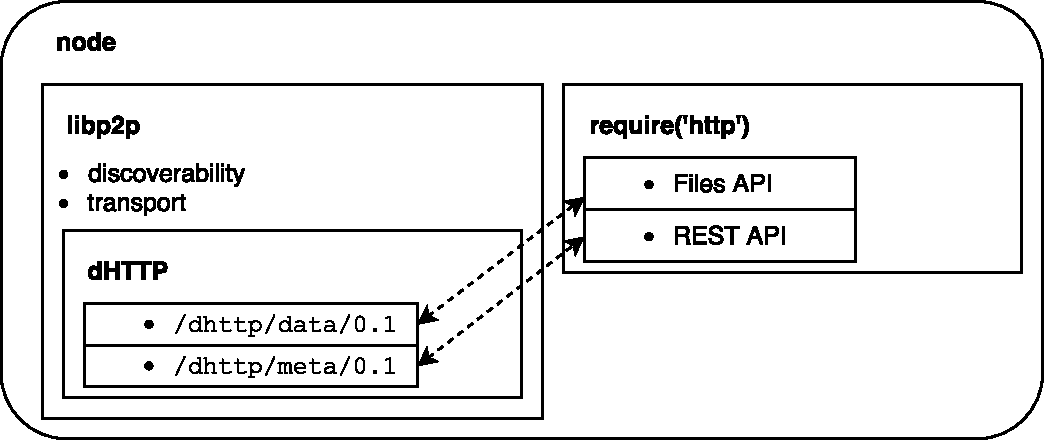
\includegraphics[scale=0.6]{nodeHiLevel.pdf}\captionof{figure}{Wizualizacja węzła dHTTP na poziomie sieci.}}

    \item Połącz się z {\em Rendezvous Server}. Prześlij informacje o swoim połączeniu i odbieraj informacje o innych węzłach sieci. \\ \parbox{\linewidth}{\centering 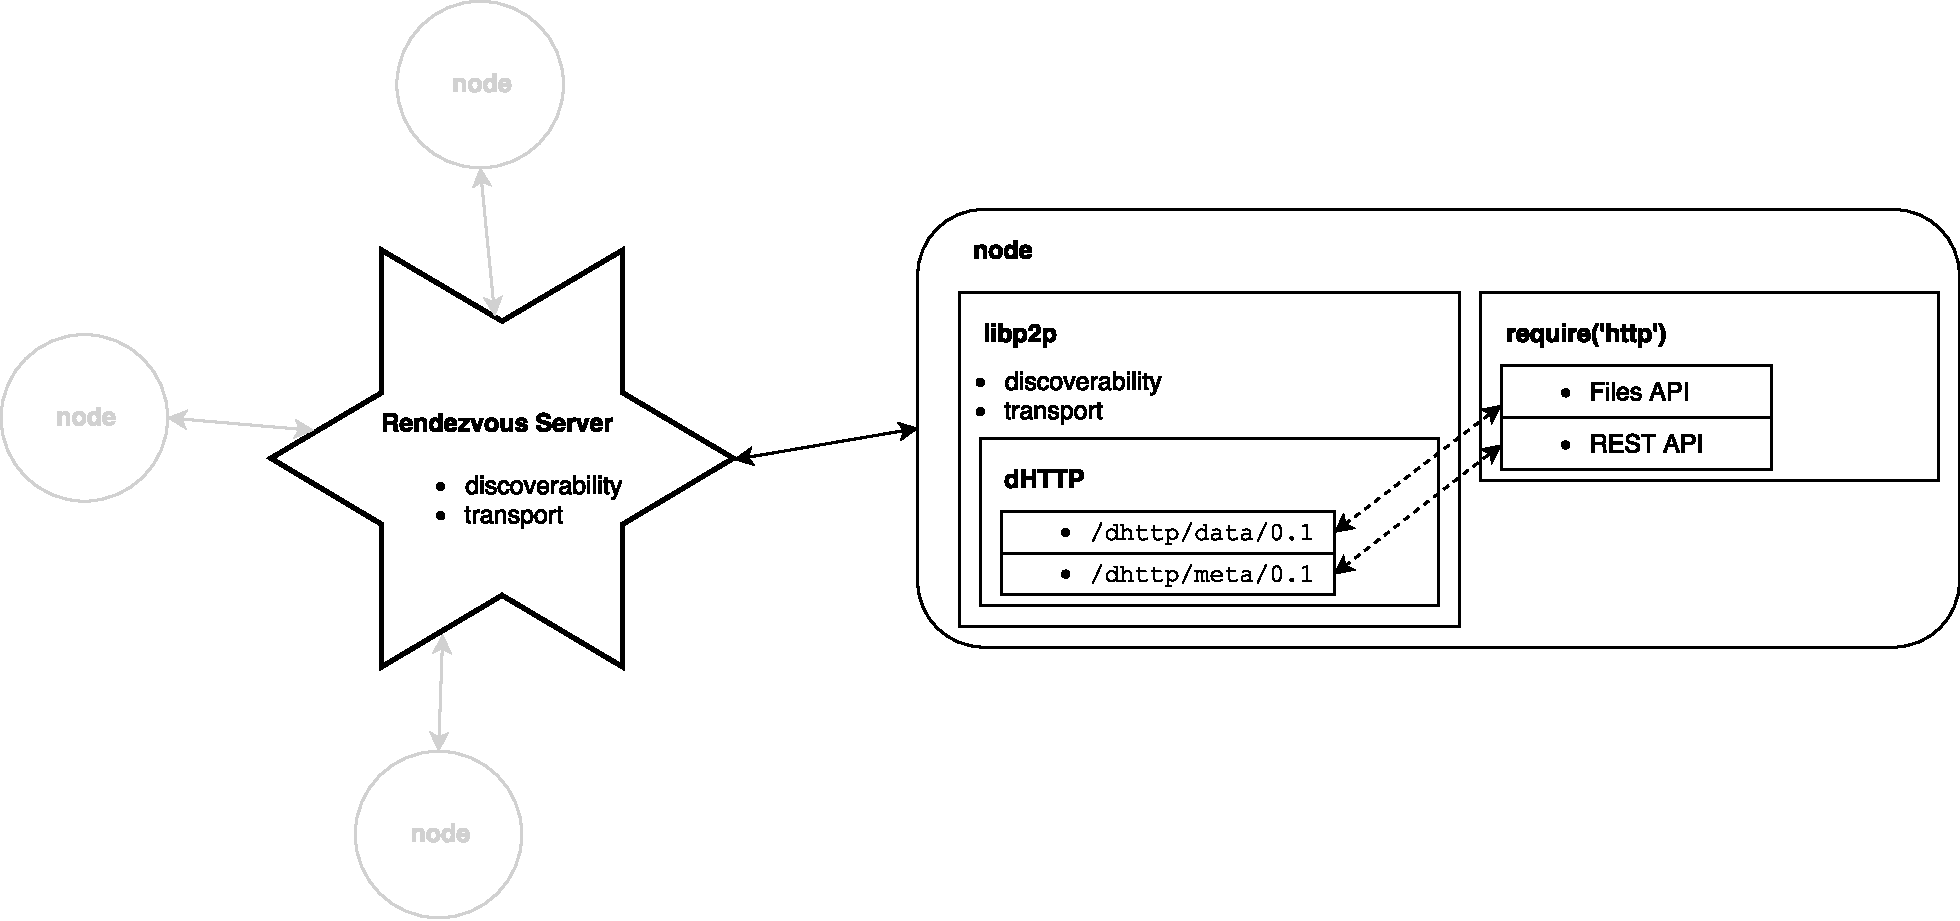
\includegraphics[scale=0.45]{node-with-rs-n-neighbors.pdf}\captionof{figure}{Wizualizacja połączenia z {\em Rendezvous Server}, posiadającego dostęp do innych węzłów sieci.}}

    \item Jeśli otrzymasz informacje o innych węzłach, utwórz z nimi połączenie i wymień się metadanymi. 

    \item Utrzymując otwarte połączenia z węzłami i uruchomiony serwer HTTP, odpowiadaj na zapytania protokołów \texttt{/dhttp/data/0.1} oraz \texttt{/dhttp/meta/0.1} i propaguj informacje zmianach zgodnie z \ref{sec:events}. \\ \parbox{\linewidth}{\centering 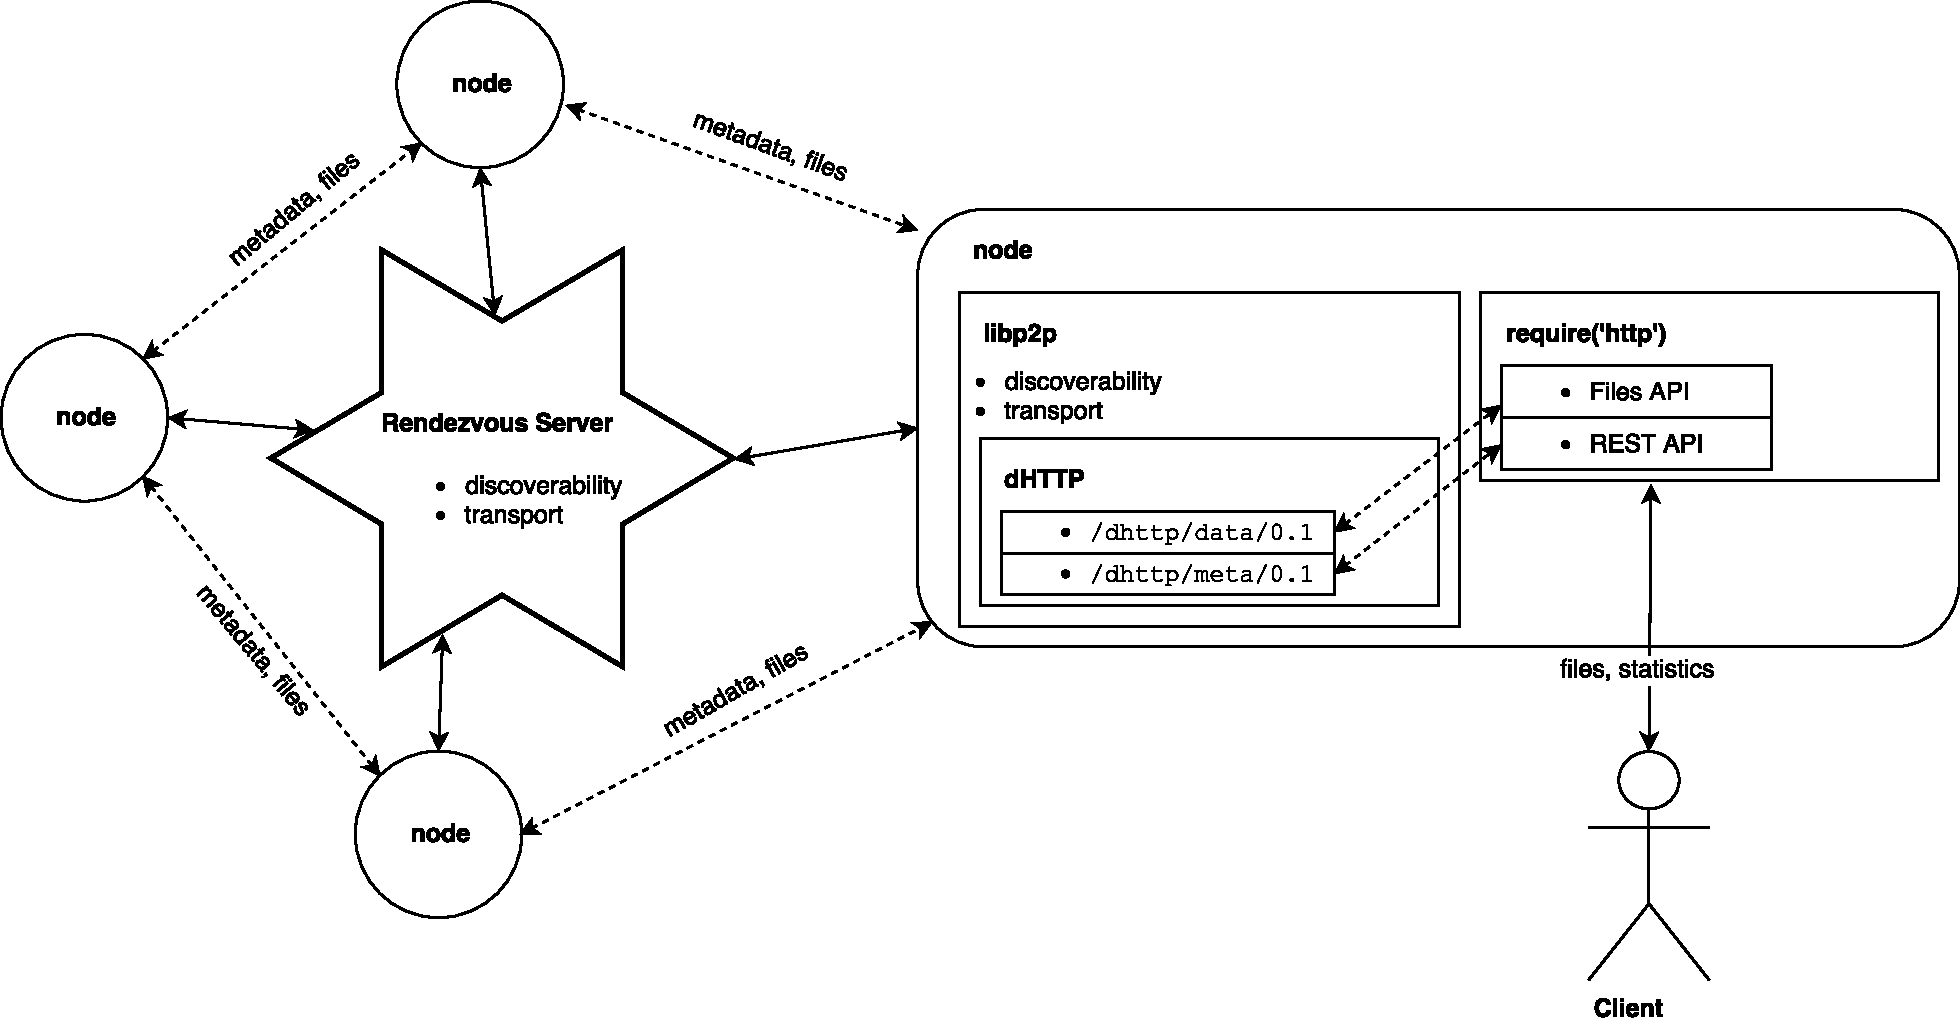
\includegraphics[scale=0.5]{communication-flow.pdf}\captionof{figure}{Wizualizacja wirtualnych połączeń między węzłami i interakcji z klientem przy użyciu API HTTP.}}
\end{enumerate}


\subsection{Przechowywanie i propagacja danych}
\label{sec:dataPropagation}

Jednym z bardziej złożonych problemów konceptu dHTTP jest kwestia przechowywania i rozpraszania plików w sieci.

Naiwne podejścia -- przechowywanie wszystkich plików na wszystkich węzłach, lub rozkładanie ich tak, aby w sieci istniał tylko jeden węzeł z danym dokumentem -- wiążą się z oczywistymi problemami: prowadzą do skrajnego przeciążenia pamięciowego w pierwszym przypadku i ryzyka dużego obciążenia pojedynczych węzłów w drugim. 

Poniżej zaproponowano kilka rozwiązań starających się znaleźć kompromis pomiędzy pamięciową złożonością sieci, a możliwością zapewniania plików przez proporcjonalną do obciążenia sieci ilość węzłów.

\subsubsection{Rozwiązanie czasu rzeczywistego}
Ideą rozwiązania jest udostępnianie plików przez dany węzeł tak długo, jak długo strona je serwująca znajduje się na ekranie klienta. Z racji swojej charakterystyki, rozwiązanie to można wykorzystać tylko na węzłach klienckich.

Zaletą jest małe obciążenie pamięciowe dla zadanego węzła i brak specjalnych metryk współdzielonych między węzłami.
Wadą -- potencjalny mały wpływ danego klienta na propagację danych w sieci, zakładając częste zmienianie wyświetlanych stron i zamykanie kart.

\subsubsection{Popularność}
To rozwiązanie polegało na serwowaniu zasobów pobranych na podstawie {\em popularity index} zawartego w sieci.

Sieć propagowałaby informacje o popularności danych stron, a pojedyncze węzły na podstawie tych informacji podejmowałyby decyzje o priorytetyzacji pobierania konkretnych plików.

Zaletą rozwiązania jest możliwość wykorzystania istniejących indeksów -- jeśli sieć będzie w początkowej fazie mała, optymalizacja typowego wykorzystania będzie możliwa dzięki zaimportowaniu zdefiniowanej listy stron, i wykorzystanie {\em web crawlingu}\footnote{Rozwiązanie polegające na rekurencyjnym przeglądaniu łącz stron internetowych w celu gromadzenia danych.} do pobrania ich zasobów przed propagacją danych o popularności wewnątrz samej sieci. Należy jednak zauważyć, że to rozwiązanie wymaga propagacji informacji o popularności plików między węzłami.

\subsubsection{Opóźnienia}
Rozwiązanie oparte na opóźnieniach może prowadzić do dobrych efektów w sieciach o niskiej przepustowości.

Idea systemu badającego opóźnienia polega na badaniu jak długo trwa typowe zapytanie o dany zasób w momencie czasu; jeżeli ta wartość jest wysoka, można założyć, że dane serwery lub węzły dHTTP są znacznie obciążone, i należy rozpropagować ich dane.

Idea ta jest najbardziej złożona algorytmicznie: należałoby przechwytywać informacje o czasach reakcji, a następnie propagować je pośród całej sieci. Uwzględnić trzeba również dynamikę ruchu internetowego -- szczyt popularności danej strony może trwać krótki czas, dane o opóźnieniach musiałyby zatem być propagowane i przechowywane w sposób tę dynamikę uwzględniający.

\subsubsection{Propagacja na podstawie zapytań}
Idea propagacji na podstawie zapytań proponuje proste rozwiązanie -- jeżeli dany węzeł zostanie zapytany o zasób i nie będzie go posiadał, zgodnie z algorytmem przedstawionym w sekcji \ref{sec:transportAlgorithm} przekieruje użytkownika do innego węzła sieci lub przekaże mu zasób bezpośrednio z serwera; robiąc to jednak, zainicjuje pobranie danego pliku u siebie, rozszerzając zasięg sieci i umożliwiając pobieranie pliku od siebie w przyszłości.

\section{Klient \texttt{dHTTP}}
Lekki klient będący wtyczką do Google Chrome udostępnia możliwość korzystania z sieci dHTTP dla zdefiniowanych typów zasobów, wykorzystując jako punkt wejścia wybrany węzeł sieci.

Wtyczka wykorzystuje udostępniane przez Google Chrome Extension API \texttt{chrome.webRequest} \cite{webRequestAPI}, pozwalające na operację podmiany adresu zapytania zanim zostanie ono wysłane na serwer; dzięki temu możliwe są przekierowania  niewymagające modyfikacji DOM-u stron internetowych, uwzględniające także asynchroniczne zapytania AJAX.

\begin{figure}[h]
	\centering
	\begin{subfigure}{1\textwidth}
		\centering
		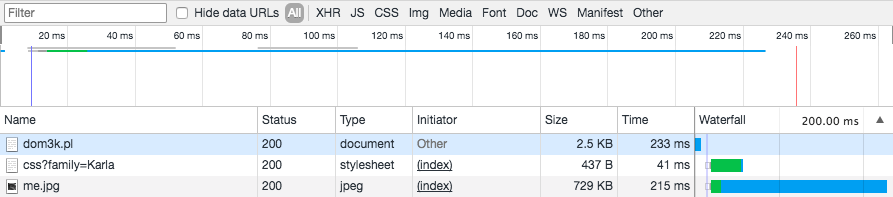
\includegraphics[scale=0.45]{no-redir.png}
		\subcaption{\label{subfigure_a}}
    \end{subfigure}
    \begin{subfigure}{1\textwidth}
		\centering
		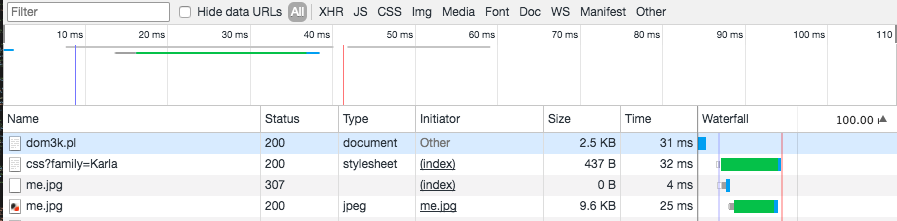
\includegraphics[scale=0.45]{redir.png}
		\subcaption{\label{subfigure_b}}
	\end{subfigure}
	
	\caption{Przykład zapytania bez przekierowania \protect\subref{subfigure_a} i zapytania, które zostało przechwycone przez wtyczkę \protect\subref{subfigure_b} -- kod HTTP 307 reprezentuje przekierowanie prowadzące do węzła dHTTP.}

\end{figure}

\begin{figure}[h]
    \centering
    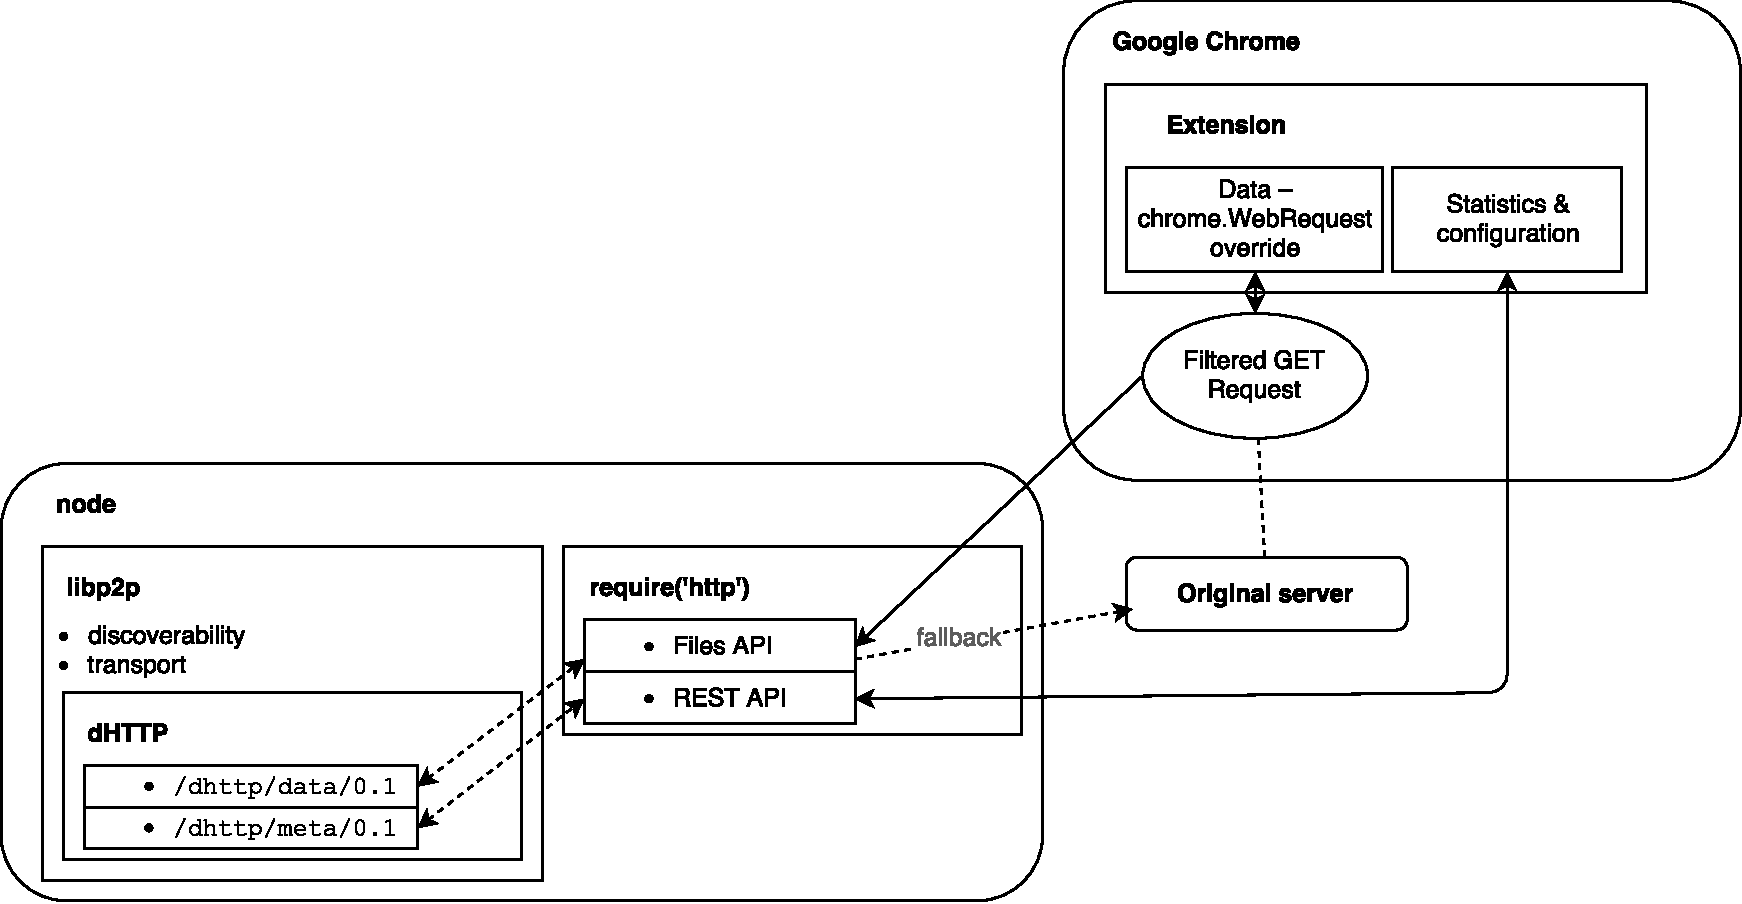
\includegraphics[scale=0.55]{client-flow.pdf}

    \caption{Wizualizacja przepływu danych przeglądarki Chrome wyposażonej w dHTTP.}
    \label{fig:client-flow}
\end{figure}

\newpage

\subsection{Eksperymentalny pełny klient}

Oryginalną ideą przyswiecającą projektowi dHTTP było udostępnienie klienta-wtyczki wyposażonego bezpośrednio w kompletny węzeł, z pominięcie pośredniego serwera node.js.

Ponieważ nie jest możliwym uruchomienie w rozszerzeniu oprogramowania serwerowego (jak \texttt{http} oferowany przez node.js), jak i tworzenie plików bezpośrednio w systemie plików użytkownika, przekierowania na adresy serwerowe nie mogłyby zostać obsłużone. Jedyną opcją pozostawało tworzenie ścieżki \texttt{data:}, co z kolei wymusza przekład danych do \texttt{base64}. Ponadto, aby wykonać tego typu zapytanie, konieczne jest sztuczne blokowanie wywołań JavaScriptowych w oczekiwaniu na zakończenie strumieni danych. API Chrome w obecnym kształcie uniemożliwia zatem realizację tego rozwiązania w sposób wydajny.

\chapter{Testy i optymalizacja}
\label{cha:testyIOptymalizacje}

\section{Zarys użytkowości i działania systemu}
\label{sec:UX}

\section{Wydajność systemu}
\label{sec:wydajnosc}

\subsection{Wydajność klienta}
\label{sec:wydajnoscKlient}

\subsection{Wydajność serwera}
\label{sec:wydajnoscNode}

\subsubsection{Wydajność rozwiązań propagacji danych}
\subsubsection{Wydajność protokołów komunikacji między węzłami}

\subsection{Proponowane rozwiązania}

\section{Podsumowanie rozwiązań optymalizacyjnych}
\label{sec:optSummary}


\chapter{Podsumowanie}
\label{cha:summary}

Celem tej pracy było opracowanie rozwiązania rozpraszającego statyczne dane stron internetowych w celu zwiększenia wydajności przeglądania. System musiał wykazać się wysoką wydajnością i prostotą użytkowania -- jest w końcu próbą uczynienia IPFS przystępnym dla użytkownika końcowego, zastosowaniem leżącej pod nim technologii w celu popularyzacji rozwiązań zdecentralizowanych.

% TODO - upewnij się co do tej wydajności x)
Testy wykazują, że w pewnych okolicznościach zastosowanie dHTTP ma zauważalny wpływ na wydajność. Dzięki swojej konstrukcji, projekt w sposób przezroczysty dla użytkownika optymalizuje sposób w jaki przegląda on często odwiedzane strony, a zdecentralizowana architektura obniża obciążenie serwerów; zwiększanie skali sieci z kolei ma pozytywny wpływ na wszystkich jej użytkowników.

\section{Potencjalne kierunki rozwoju}
\label{sec:future}

Zaprezentowany projekt nie wyczerpuje możliwości rozwoju.

Choć wstępne eksperymenty okazały się mieć satysfakcjonujące wyniki, trudno ocenić  sprawność systemu wielkiej skali na podstawie tak małej próby. W celu faktycznej walidacji utworzonych rozwiązań, konieczne będą ekstensywne testy, które mogą doprowadzić do istotnych wniosków. Wydajność sieci mogłaby również zostać znacznie poprawiona dzięki rozwojowi algorytmów zaproponowanych w sekcji \ref{sec:dataPropagation}, zapewniających optymalniejszy rozkład danych w sieci.

Kluczowe dla trafienia do szerokiego grona odbiorców może być pokonanie ograniczeń narzucanych przez API Google Chrome. W obecnym kształcie wymusza ono instalację osobnego oprogramowania w celu uruchomienia węzła sieci, co jest problematyczne dla większości użytkowników internetu.


% itd.
% \appendix
% \include{dodatekA}
% \include{dodatekB}
% itd.

%  TODO - upewnij się, że InProceedings drukuje URLe.

\printbibliography

\end{document}
